\input{../header}
\rhead{Your name: \rule{8cm}{0.15mm}}

\begin{document}


\section{Learning target AD8, version 1}

Model and analyze scenarios using applied optimization.

{\tiny Hints: Draw three pictures; label variables and constants; write a constraint equation; write an objective function that just has one variable; find any endpoints; do the finding extrema recipe.}

\hrulefill

You are a dinosaur rancher, and you need to build pens for your three dinosaurs. You decide to build an electric fence around a rectangular region with total area of 25 square kilometers, and then separate this region into three equal-size rectangular pens with two more strips of electric fence. What's the minimum length of electric fencing you need to do this? 

\vspace{1em}

%Make sure to do all six steps of the appropriate recipe. 
Here is one of your three pictures.
\[
	\begin{tabular}{|l|c|c|}
		\hline
 		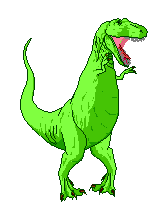
\includegraphics[width=1in]{../images/t-rex.png} & 
 		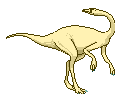
\includegraphics[width=1in]{../images/dromiceiomimus.png} &
 		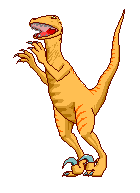
\includegraphics[width=1in]{../images/utahraptor.png} \\
		\hline
		% I need a padding row
		\multicolumn{1}{l}{} & \multicolumn{1}{l}{} & \multicolumn{1}{l}{} 
	\end{tabular}
\]
\vfill



The minimum length of fence is $\underbrace{\qquad\qquad}_{\text{number}}$ $\underbrace{\quad}_{\text{units}}$, 

and the dimensions of the dinosaur pen that make this work are 
$\underbrace{\qquad\qquad}_{\text{number}}\, 
\underbrace{\quad}_{\text{units}}
\times 
\underbrace{\qquad\qquad}_{\text{number}}\,
\underbrace{\quad}_{\text{units}}$.

%%%%%%%%%%%%%%%%%%%%%%%%%%%%%%%%%%%%%%%%%%%%%%%%%%%%%%%%%
\pagebreak
%%%%%%%%%%%%%%%%%%%%%%%%%%%%%%%%%%%%%%%%%%%%%%%%%%%%%%%%%


\section{Learning target AD8, version 2}

Model and analyze scenarios using applied optimization.

\hrulefill

If you take a regular 8.5" x 11" sheet of paper and cut squares out of the corners, you can fold up the flaps on all four sides to make a box (without a lid). How large should you cut the squares so that the resulting box has maximum volume?

{\tiny Hints: Draw three pictures; label variables and constants; write a constraint equation; write an objective function that just has one variable; find any endpoints; do the finding extrema recipe.}

\vfill

The maximum volume is $\underbrace{\qquad\qquad}_{\text{number}}$ $\underbrace{\quad}_{\text{units}}$, 

and the dimensions of the box that make this work are 
$\underbrace{\qquad\qquad}_{\text{number}}\, 
\underbrace{\quad}_{\text{units}}
\times 
\underbrace{\qquad\qquad}_{\text{number}}\,
\underbrace{\quad}_{\text{units}}
\times
\underbrace{\qquad\qquad}_{\text{number}}\,
\underbrace{\quad}_{\text{units}}$.

\end{document}

NOTE: Any combination of circle, square, and eq. triangle (area = \frac{\sqrt{3}}{4}t^2) gives nice behavior for the piece-of-wire context.